\begin{figure}[htbp]
\centering
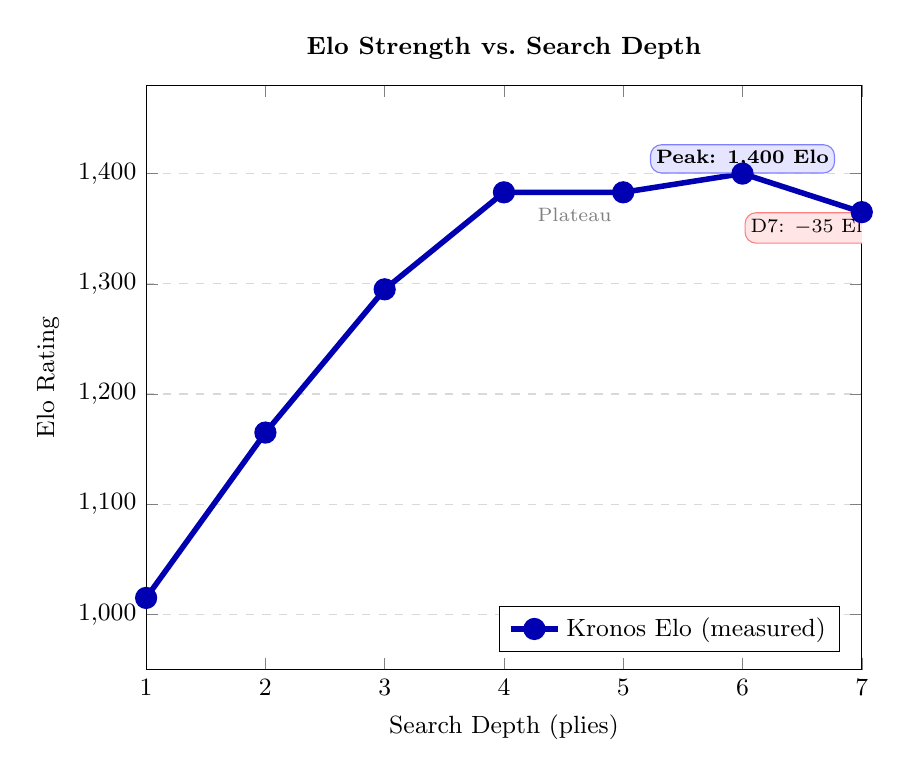
\begin{tikzpicture}
\begin{axis}[
    title style={font=\bfseries\small},
    title={Elo Strength vs.\ Search Depth},
    xlabel={Search Depth (plies)},
    ylabel={Elo Rating},
    xmin=1, xmax=7,
    ymin=950, ymax=1480,
    xtick={1,2,3,4,5,6,7},
    ytick={1000,1100,1200,1300,1400},
    legend pos=south east,
    ymajorgrids=true,
    grid style={dashed, gray!30},
    width=0.88\textwidth,
    height=9cm,
    tick label style={font=\small},
    label style={font=\small},
    legend style={font=\small},
    nodes near coords style={font=\scriptsize}
]
\addplot[
    color=blue!70!black,
    mark=*,
    mark size=3pt,
    line width=2pt
]
coordinates {
    (1, 1015)
    (2, 1165)
    (3, 1295)
    (4, 1383)
    (5, 1383)
    (6, 1400)
    (7, 1365)
};

\addlegendentry{Kronos Elo (measured)}

% Peak label
\node[font=\scriptsize, fill=blue!10, draw=blue!50, rounded corners, inner sep=2pt,
      anchor=south] at (axis cs:6,1400) {\textbf{Peak: 1{,}400 Elo}};

% Regression label
\node[font=\scriptsize, fill=red!10, draw=red!50, rounded corners, inner sep=2pt,
      anchor=north] at (axis cs:7,1365) {D7: $-$35 Elo (timeout)};

% D5 plateau label
\node[font=\scriptsize, text=gray, anchor=north west] at (axis cs:4.2,1378) {Plateau};

\end{axis}
\end{tikzpicture}
\caption[Elo Playing Strength vs. Search Depth]{Elo rating scaling as a function of search depth, showing peak calibrated strength at depth 6. The regression at depth 7 results from worker timeout-induced search aborts.}

\label{fig:strength_vs_depth}
\end{figure}
% Source Material: cross_depth_elo.tex table data
